\documentclass[11pt, aspectratio=169]{beamer}
\usepackage[french,noconfigs]{babel}
\usepackage{presentation/beamerx}
  \setbeamercovered{invisible}
\usepackage{presentation/jonas}

\graphicspath{
    {img/code/}              % Figures produced by me, with cod from the repo.
    {img/extern/}            % Figures that I did not create myself
    {img/extern/beamerx/}   % Necessary for the theme.
}
% \newcommand*\InputBiasTable[1]{\input{img/bias_tables/#1}}
\newcommand*\InputBiasTable[1]{\input{img/code/#1}}

\title[EPS-HEP2021]{
    A combined fit to the Higgs Branching Ratios at ILD
}[Combined Higgs fit]
\author[Jonas Kunath]{Jonas Kunath (LLR), on behalf of the ILD concept group}
\date{29.07.2021}

\begin{document}
\maketitle
\xsection{myblue}{Intro\-duction}
    \begin{frame}
    \frametitle{The International Linear Collider (ILC)}
    \begin{columns}[c,onlytextwidth]
    \begin{column}{0.60\textwidth}
        \begin{itemize}
            \item Linear $e^+e^-$ collider.
            \item Polarized beams.
            \item Initial stage $\sqrt{s} = 250~\GeV$ (considered here).
            \item Upgradable (350~\GeV, 500~\GeV, 1~TeV).
        \end{itemize}
        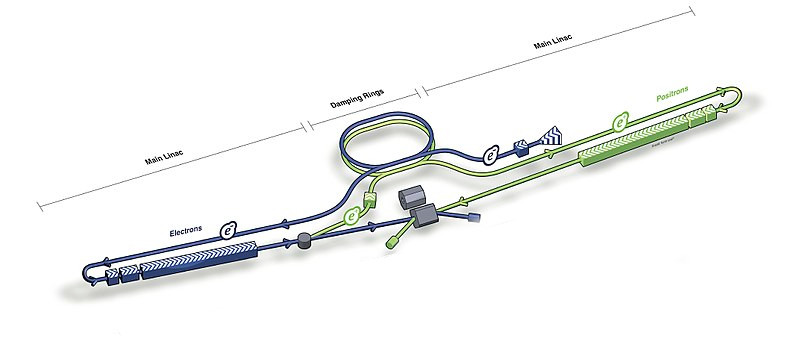
\includegraphics[height=0.4\textheight, width=\textwidth, keepaspectratio]{pr_ILC_SchemeTDR}
    \end{column}
    \begin{column}{0.40\textwidth}
    \begin{tikzpicture}[remember picture,overlay]
        \node[anchor=north west,inner sep=0pt] at ($(current page.center) + (1.5,2.5)$) {
            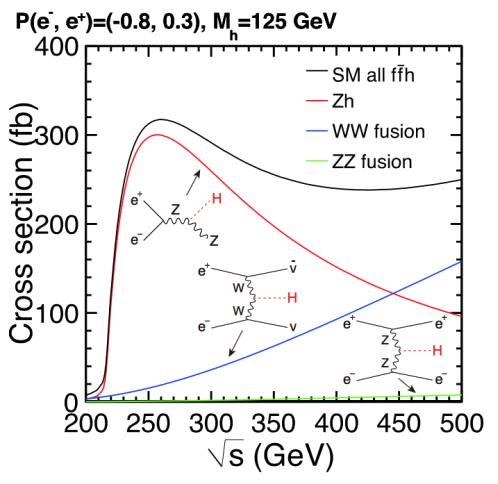
\includegraphics[height=0.6\textheight, width=\textwidth, keepaspectratio]{IGP_xsec_h_ILC_left}
        };
    \end{tikzpicture}
    \end{column}
    \end{columns}
    \vfill
    {\footnotesize
    \href{https://linearcollider.org/technical-design-report/}{ILC Technical Design Report (2013)}\newline
    The International Linear Collider: A Global Project:
    \href{https://arxiv.org/abs/1903.01629}{\color{llblue}\texttt{arXiv:1903.01629}}
    }
    \end{frame}

    \begin{frame}
    \frametitle{The International Large Detector (ILD)}
    \begin{columns}[c,onlytextwidth]
    \begin{column}{0.5\textwidth}
    Based on the Particle Flow approach.
    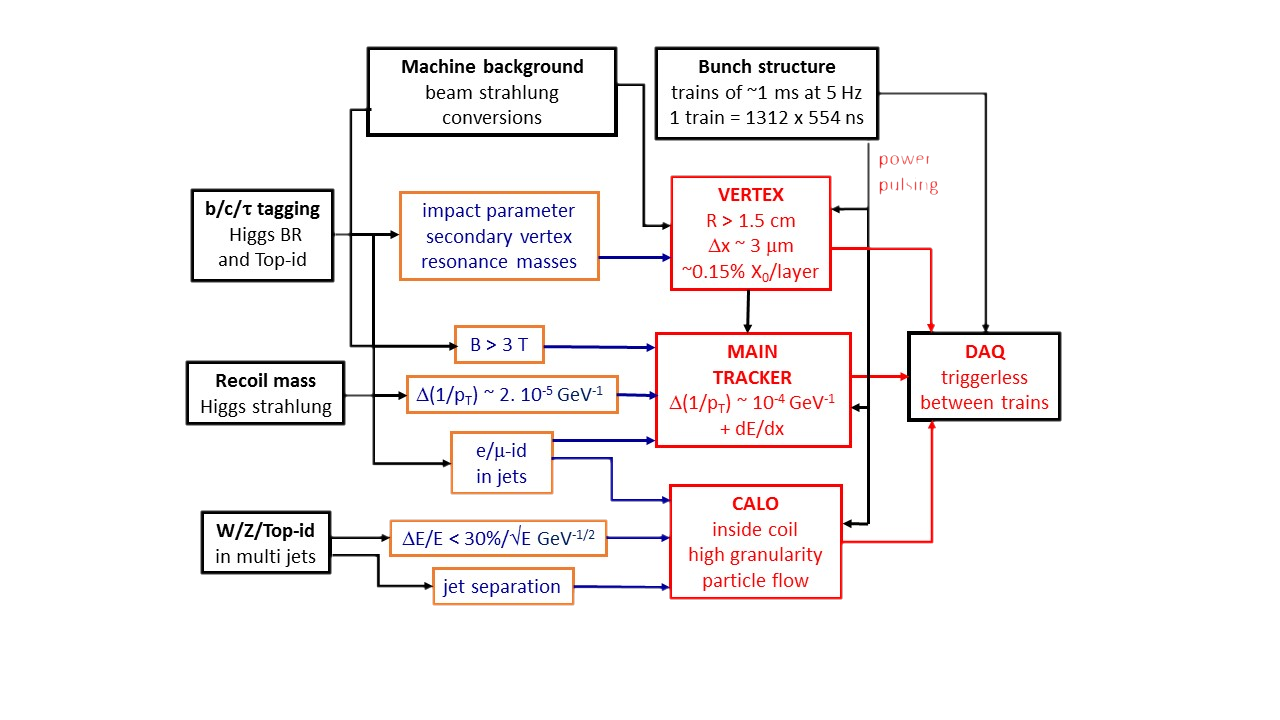
\includegraphics[height=0.6\textheight, keepaspectratio]{IDR_ILD_specifications}
    \vfill
    {\footnotesize
    Interim Design Report:
    \href{https://arxiv.org/abs/2003.01116}{\color{llblue} \texttt{arXiv:2003.01116}}
    }
    \end{column}
    \begin{column}{0.5\textwidth}
    \resizebox{\textwidth}{!}{
    \begin{tabular}{cc}
        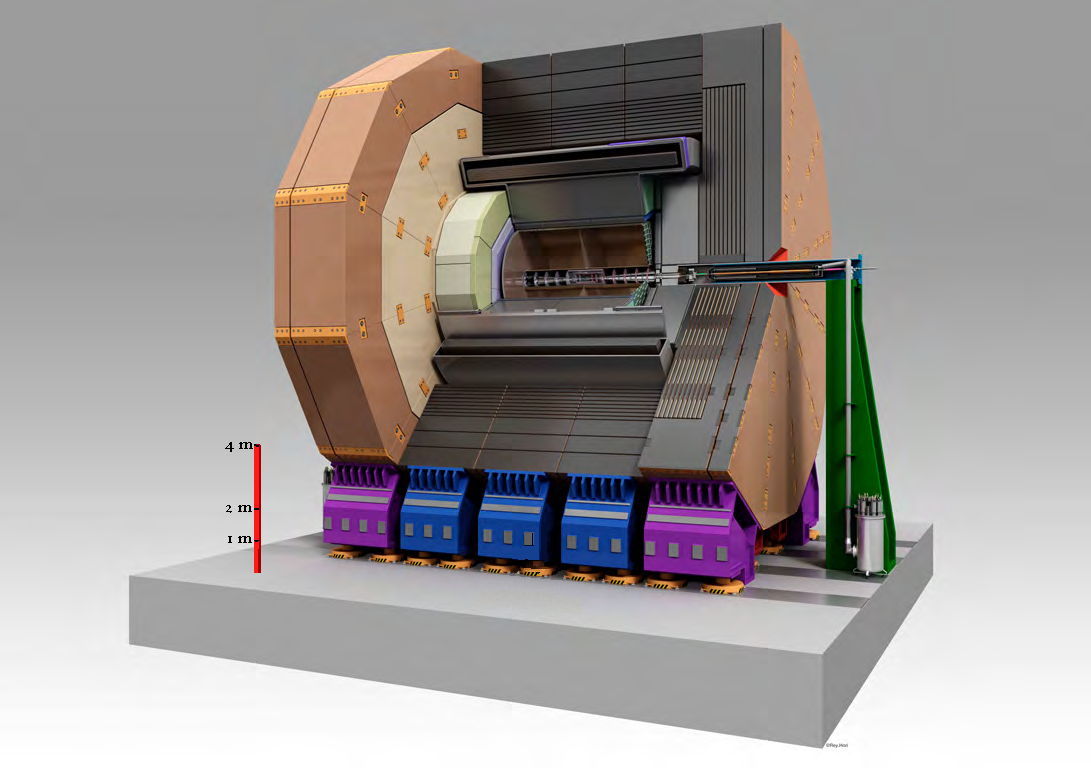
\includegraphics[width=\textwidth]{IGP_ILD}  \\
        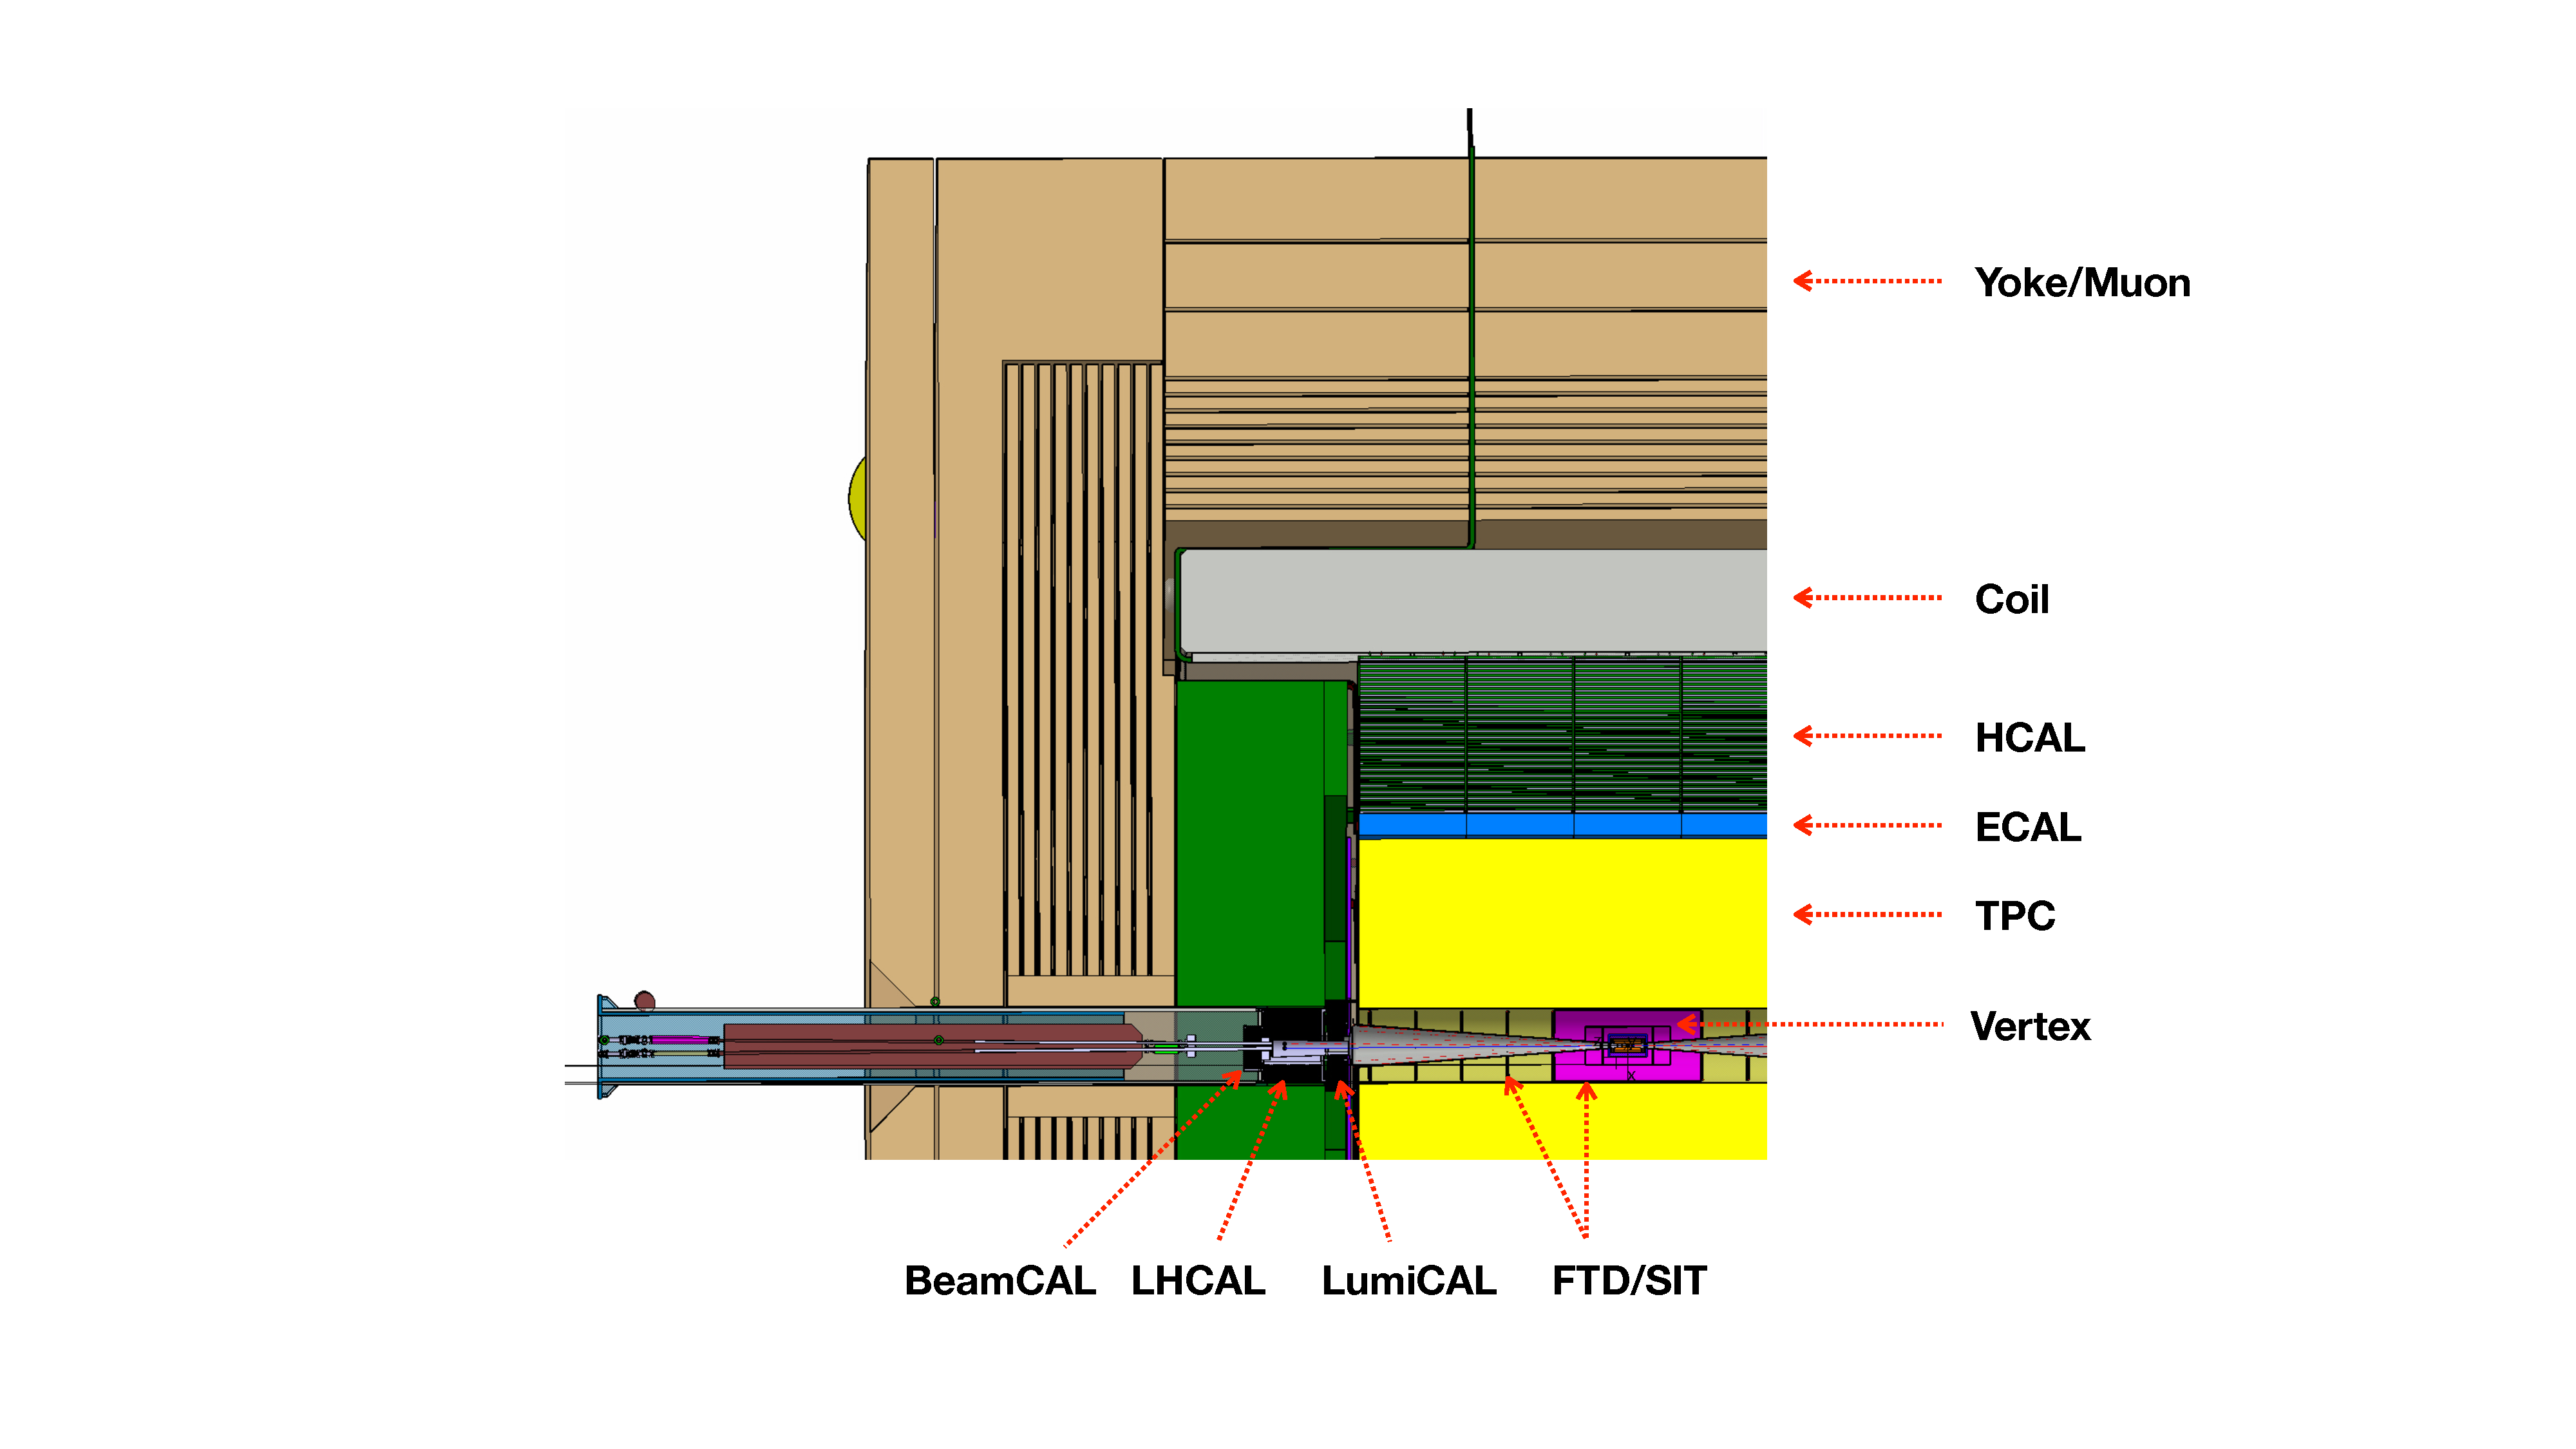
\includegraphics[width=\textwidth]{IDR_ILD_quadrant_new_lstar} &
        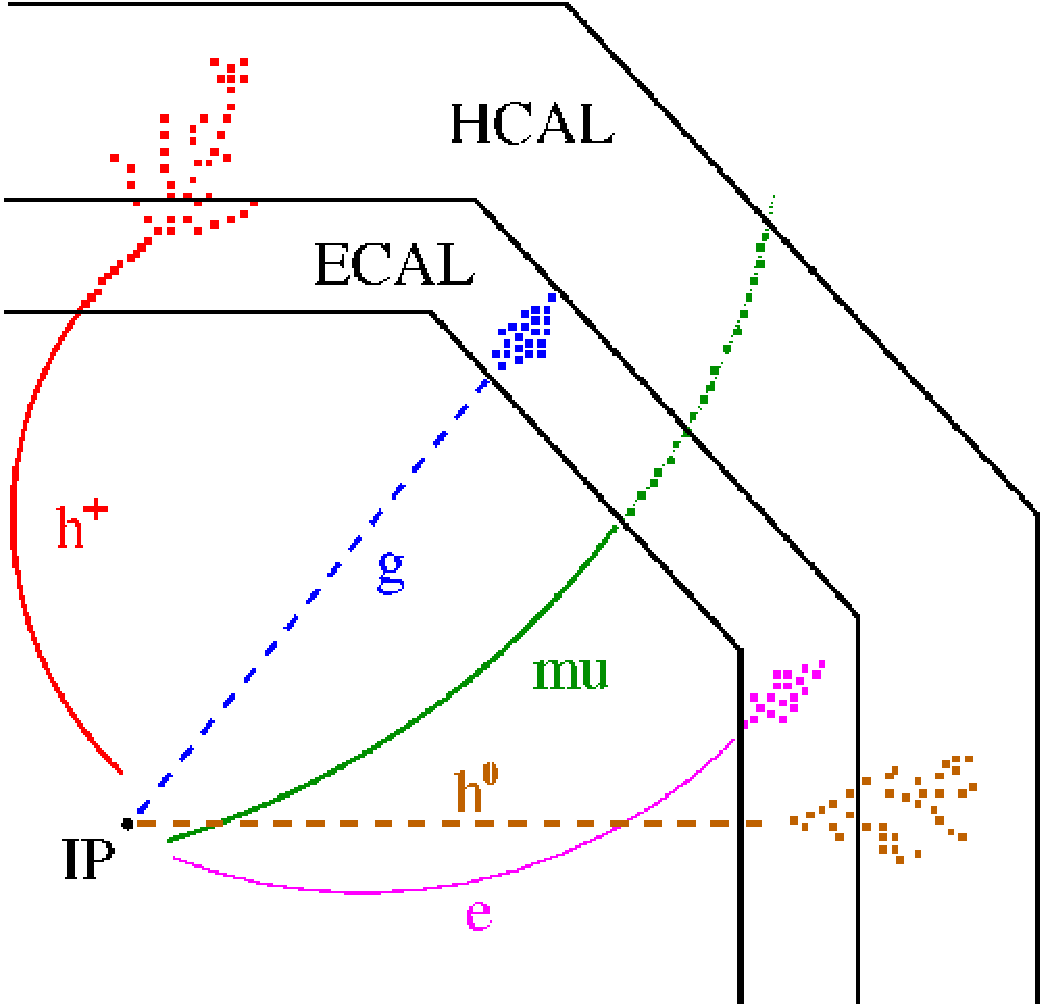
\includegraphics[width=0.75\textwidth]{ext_PFlowBasic} \\
    \end{tabular}
    }
    \end{column}
    \end{columns}
    \end{frame}

    \begin{frame}
    \frametitle{Higgsstrahlung}
    \begin{columns}[c,onlytextwidth]
    \begin{column}{0.38\textwidth}
    \resizebox{\textwidth}{!}{\FeynmanHiggsstrahlung}
    \end{column}
    \begin{column}{0.62\textwidth}
    \begin{itemize}
        \item \textcolor{xemphcolor}{
            $Z \rightarrow \mu^+ \mu^-, Z \rightarrow e^+ e^-$}:


            \begin{itemize}
                \item IsolatedLeptonTagger: \\
                    Lepton pair with same type and opposite charge.
                \item Final state radiation: \\
                    Add photons with $\cosTheta{l\gamma} > 0.99$.
            \end{itemize}
            Golden channels due to recoil mass method,
            $M_{\tn{recoil}}^2 = s + M_Z^2 - 2\sqrt{s} \cdot E_Z$.
        \item \textcolor{xemphcolor}{Higgs}:

            Event selection that keeps events with all Higgs decays.
    \end{itemize}
    \end{column}
    \end{columns}
    \end{frame}

\xsection{myblue}{Event selection}
    \begin{frame}{Event selection}
    \begin{columns}[c, onlytextwidth]
    \foreach \x in {1, ..., 5}{\only<\x>{
    \begin{column}{0.4\textwidth}
        \small Selection only on information from decay of the primary Z boson.
    \includegraphics[height=0.9\textheight, width=0.95\textwidth, keepaspectratio]
        {presel_e2e2_eff_\x}
        {\footnotesize Step 0: Find a lepton pair.}
    \end{column}
    \begin{column}{0.5\textwidth}
        \vspace{-0.1\textheight}
        \begin{center}
        \includegraphics[height=\textheight, width=\textwidth, keepaspectratio]
        {presel_e2e2_\x}
        \end{center}
    \end{column}
    \begin{column}{0.1\textwidth}
    \end{column}
    }}
    \end{columns}
    \end{frame}

\xsection{myblue}{Idea}
    \begin{frame}
    \frametitle{Higgs-BRs all-in-one}
    \setbeamercovered{transparent}
    \begin{columns}[c,onlytextwidth]
    \begin{column}{0.55\textwidth}
    \vfill
    \begin{enumerate}
        \item Build samples with all Higgs decay modes
            (Higgsstrahlung, $Z\to (e^+e^-, \mu^+\mu^-)$).
        \item<2-> Construct categories to separate the decay modes (\& background)
            as well as possible.
        \item<5-> Fit the Higgs branching ratios to the observed category counts.
    \end{enumerate}
    \end{column}
    \begin{column}{0.45\textwidth}
    \only<1>{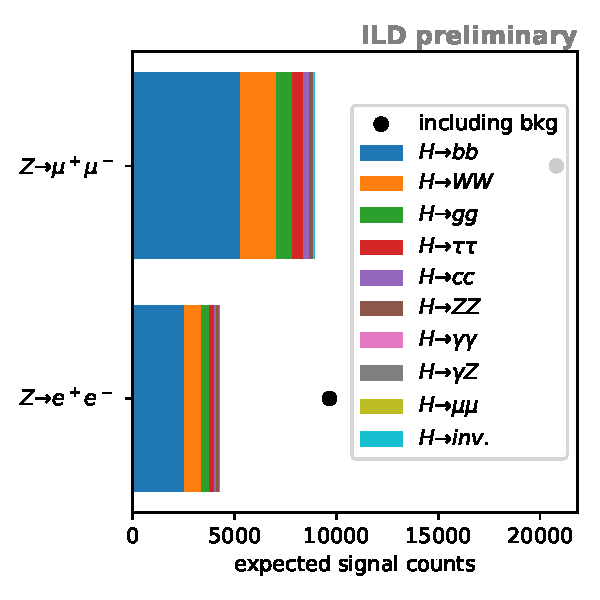
\includegraphics[height=0.75\textheight, width=0.95\textwidth, keepaspectratio]
        {intro_sample_counts}}
    \only<2>{\addtocounter{framenumber}{1} \put(0, 0){
        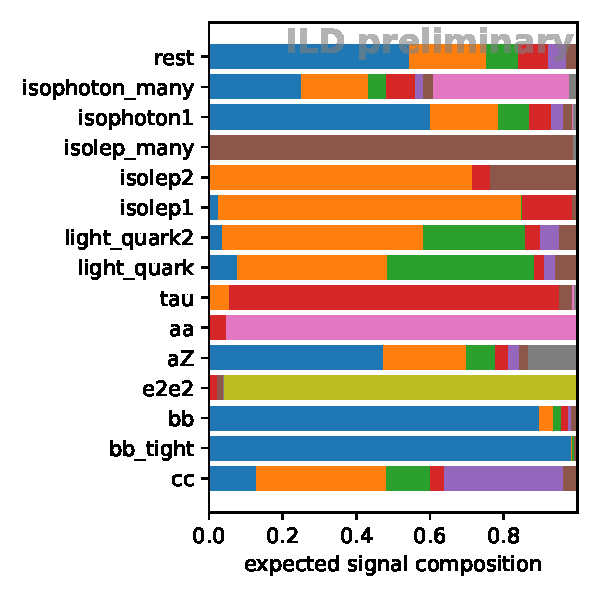
\includegraphics[height=0.75\textheight, width=0.95\textwidth, keepaspectratio]
        {intro_signal_composition_per_category}}}
    \only<3>{\addtocounter{framenumber}{1} \put(0, 0){
        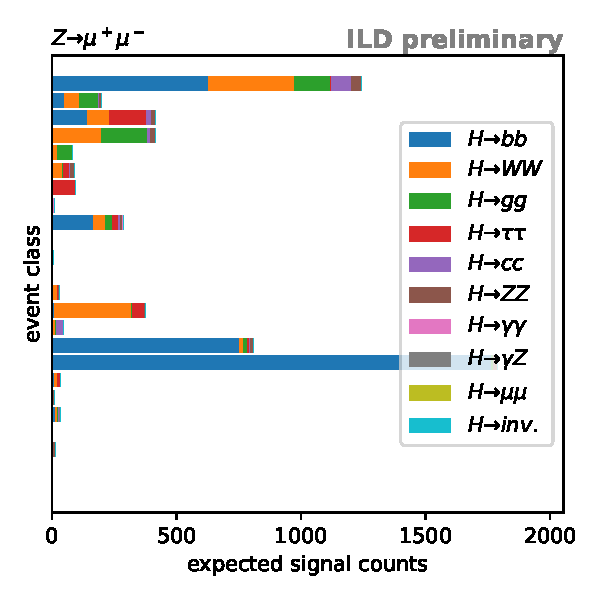
\includegraphics[height=0.75\textheight, width=0.95\textwidth, keepaspectratio]
        {intro_category_counts}}}
    \only<4>{\addtocounter{framenumber}{1} \put(0, 0){
        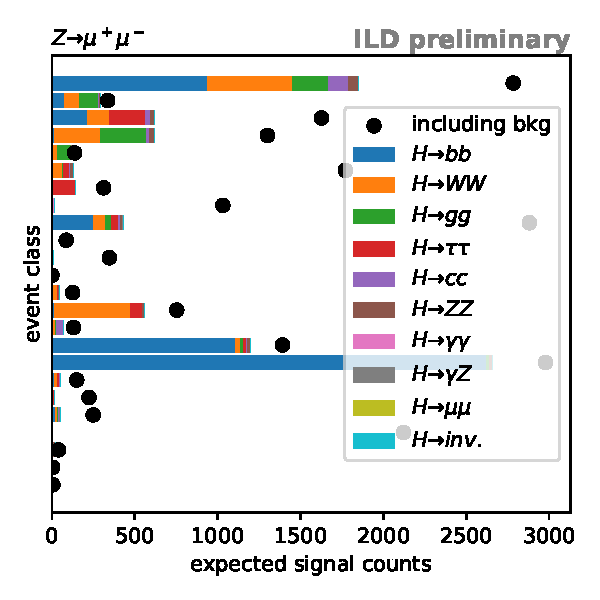
\includegraphics[height=0.75\textheight, width=0.95\textwidth, keepaspectratio]
        {intro_category_counts_w_bkg}}}
    \only<5>{\addtocounter{framenumber}{1} \put(0, 0){\centering
        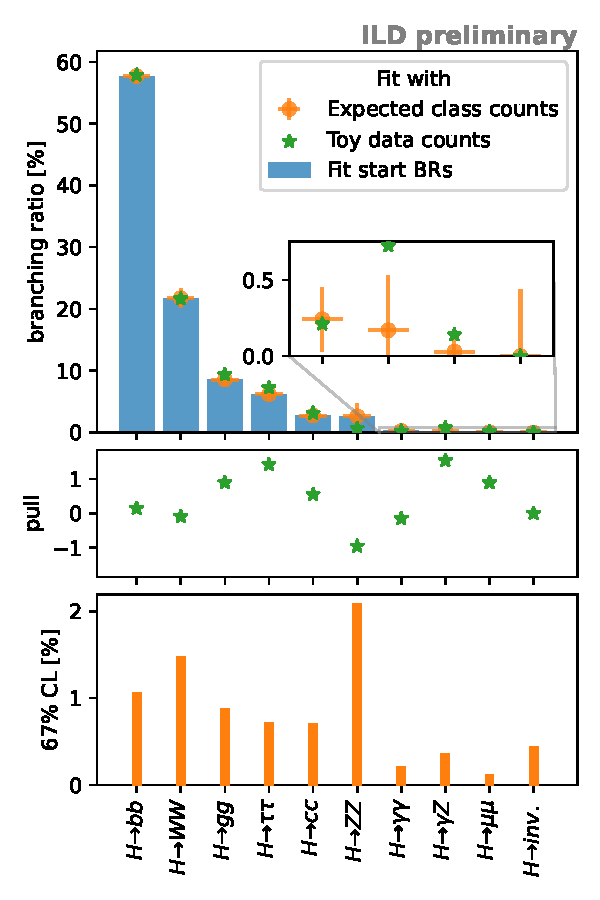
\includegraphics[height=0.9\textheight, keepaspectratio]
        {br_estimates_default}}}
    % \only<5>{\addtocounter{framenumber}{1}
    % \\
    % \textbf{Advantages}
    % \begin{itemize}
    %     \item A model independent extraction of all branching ratios (at once).
    %     \item Independent of any Higgs production cross section measurement.
    %     \item Gaussian errors $\rightarrow$ multinomial errors, as everything is in the same sample.
    %     \begin{itemize}
    %         \item Promising e.g. for $H \to b\bar{b}$.
    %             See \emph{\ref{many_likelihoods_optimizations} in backup.
    %     \end{itemize}
    %   \end{itemize}}
    \end{column}
    \end{columns}
    % {\small
    % Similar to a $\tau$ branching ratio analysis at ALEPH:
    % \href{https://arxiv.org/abs/hep-ex/0506072}{\emph{\texttt{arXiv:hep-ex/0506072}}}.
    % }
    \end{frame}

\xsection{myblue}{Implemen\-tation}
    \begin{frame}
    \frametitle{Implementation within ILC}
    Reconstructed events from $\sqrt{s} = 250~\GeV$ MC2020 ILD mass production.
    % (\texttt{ILD\_l5\_o1\_v02}, \texttt{v02-02}).
    \begin{itemize}
        \item $\sqrt{s} = 250~\GeV$ ideal for the Higgsstrahlung process.
        \begin{itemize}
            \item $Z \to e^+ e^-$ and $Z \to \mu^+ \mu^-$ as signal channels.
            \item $\geq 400$k simulated events/Standard Model decay mode.
        \end{itemize}
        \item Considered backgrounds: Standard model processes \\
            with 2 or 4 fermions in the final state.
        \item For FCC Workshop: Unpolarized beams.
        \item 2000~fb$^{-1}$ integrated luminosity.
    \end{itemize}
    \end{frame}

\xsection{myblue}{Fit}
    \begin{frame}{Optimization - Setup}
    \begin{columns}[c,onlytextwidth]
    \begin{column}{0.6\textwidth}
    BRs from minimization through
    \texttt{MINUIT}/{\emph{\href{https://github.com/scikit-hep/iminuit}{iminuit}}}.
    \begin{itemize}
        \item \texttt{MC2}:
              % Events that are (statistically) independent from \texttt{MC1}.
              Will be replaced by the detector data.
        \item $\vec{S} = M \cdot \vec{B} = \vec{f}(\vec{B})$, with
        \begin{itemize}
            \item $\vec{S}$: The signal counts per category ($S = data - bkg$). \texttt{MC2}.
            \item $M$: The matrix built from simulated events, as outlined above. \texttt{MC1}.
            \item $\vec{B}$: The target.
                  Use e.g. the Standard Model BRs as fit starting values.
        \end{itemize}
    %    \item The cost function: Currently Least Squares.
    %     \begin{itemize}
    %        \item $S$: The 1$\sigma$ binomial uncertainties on $S$ are the
    %             (only) place where the integrated luminosity effects the analysis.
    %        \item $M$:  Least Squares is not ideal: We discard known information
    %         (the total number of events in the sample).
    %     \end{itemize}
        \item The cost function: Multinomial log-likelihood.
        \begin{itemize}
            \item $- \tn{ln}\mathcal{L} = - N_{\tn{data}} \sum_i S_i \tn{ln}\left(\sum_j M_{ij}B_j\right)$.
            \item $B_{H \to ZZ^*} = 1 - \sum_{i \neq H \to ZZ^*} B_i$.
            % \item Each BR constrained to $\left[0, 1\right]$.
        \end{itemize}
    \end{itemize}
    \end{column}
    \begin{column}{0.4\textwidth}
    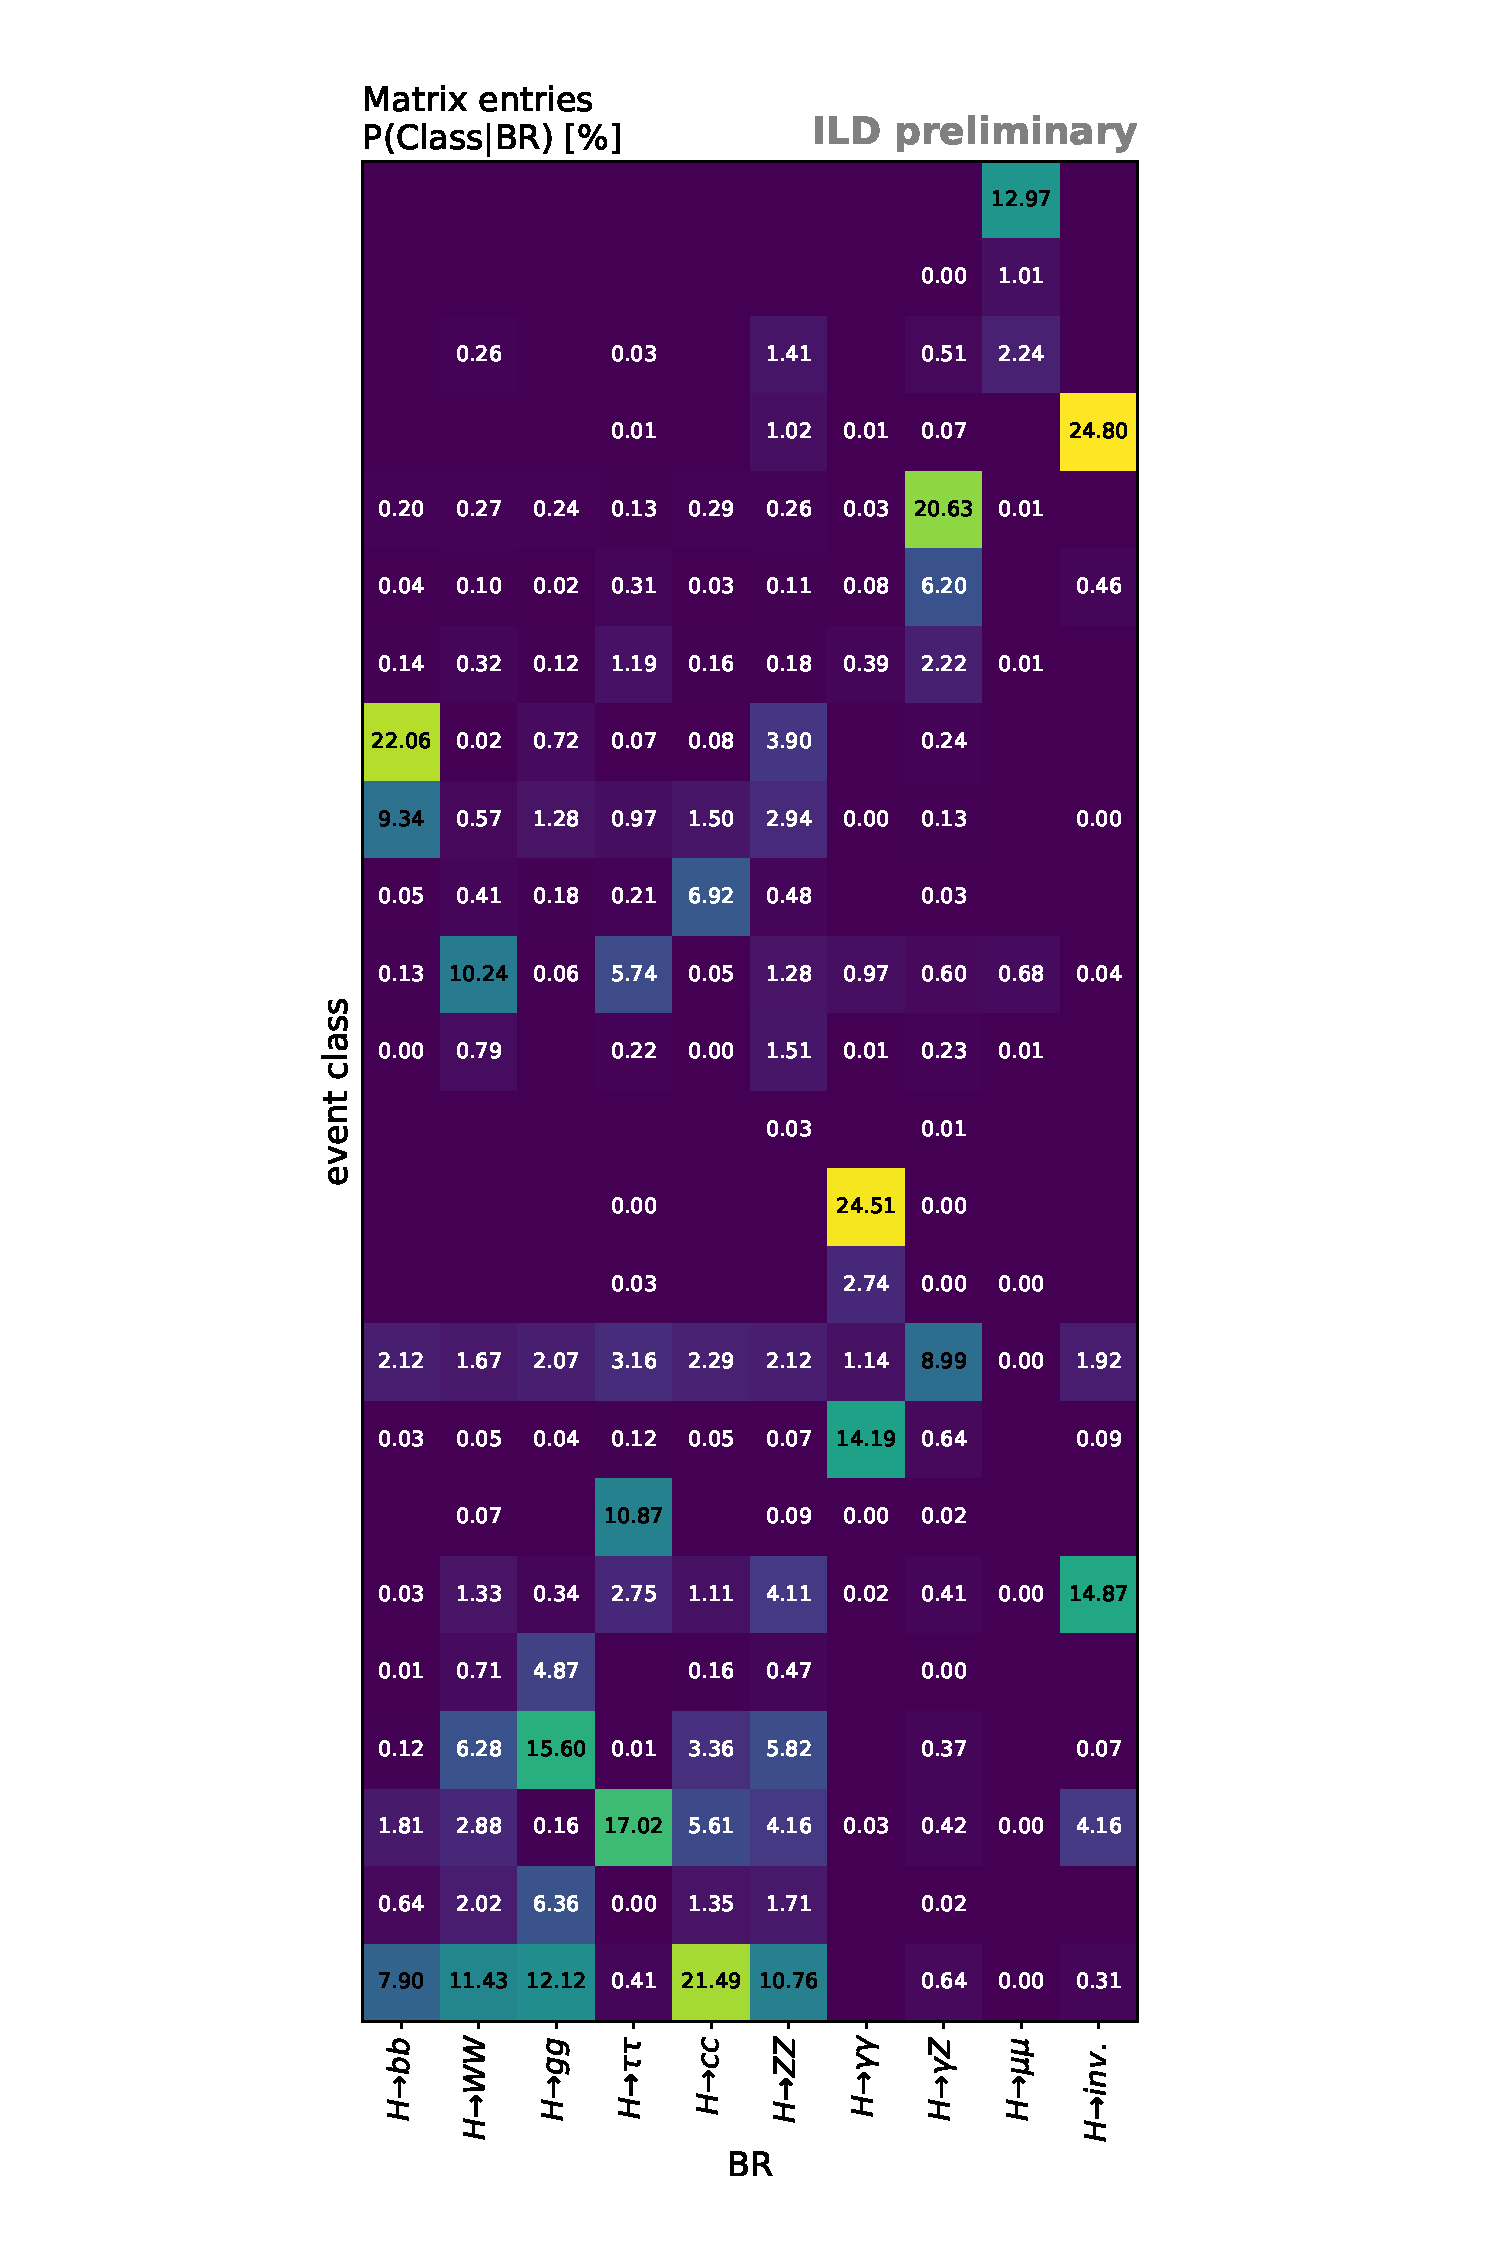
\includegraphics[height=0.85\textheight, width=0.95\textwidth, keepaspectratio]
        {probability_matrix}
    \end{column}
    \end{columns}
    \end{frame}

    \begin{frame}{Optimization - Results}
    \begin{columns}[c, onlytextwidth]
    \begin{column}{0.6\textwidth}
    The fitted BR$^{\tn{min}}$ reproduces BR$^{\tn{true}}$ within its uncertainties.
    $\sigma_{B_{H \to ZZ^*}}$ through uncertainty propagation.
    % See \emph{\\ref{correlations} in backup.
    \\
    \centering
    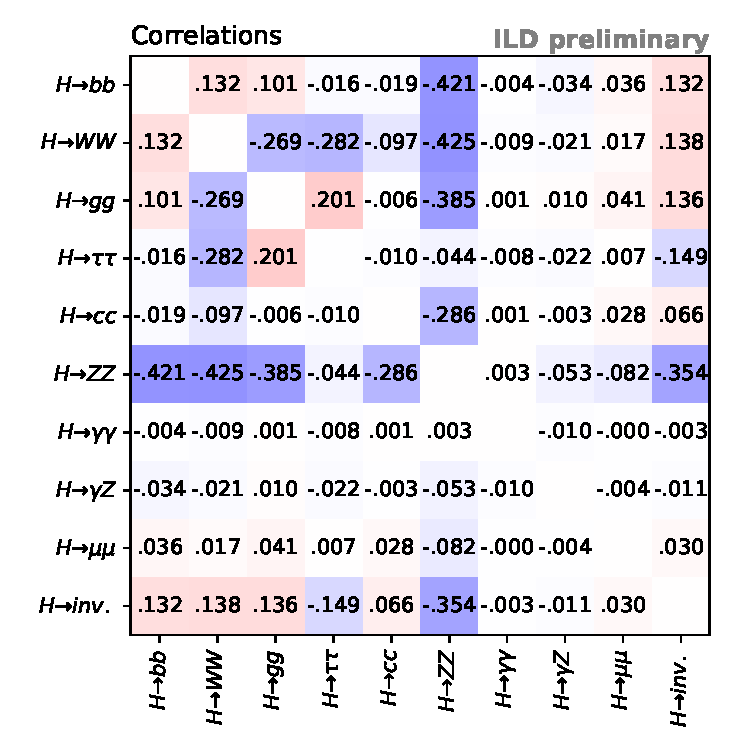
\includegraphics[width=0.8\textwidth,height=0.7\textheight, keepaspectratio]
        {correlations_default}
    \\
    \end{column}
    \begin{column}{0.38\textwidth}
    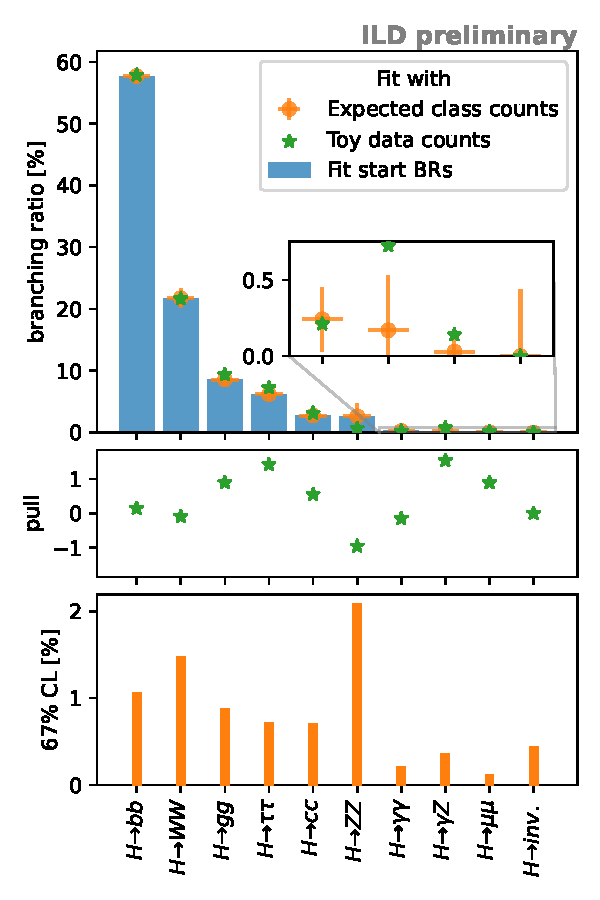
\includegraphics[height=0.85\textheight, width=0.95\textwidth, keepaspectratio]
        {br_estimates_default}
    \end{column}
    \end{columns}
    \end{frame}

    \begin{frame}{Optimization - Validity check}
    Toy study: Draw from multinomial ($N_{\tn{data}}$ fixed).
    \\
    Shown: 2 of the toy fit distributions for multinomial
    $\tn{ln}\mathcal{L}$ with $\left[0, 1\right]$ boundaries.
    \vspace{-0.5\baselineskip}
    \begin{columns}[c, onlytextwidth]
    \begin{column}{0.5\textwidth}
    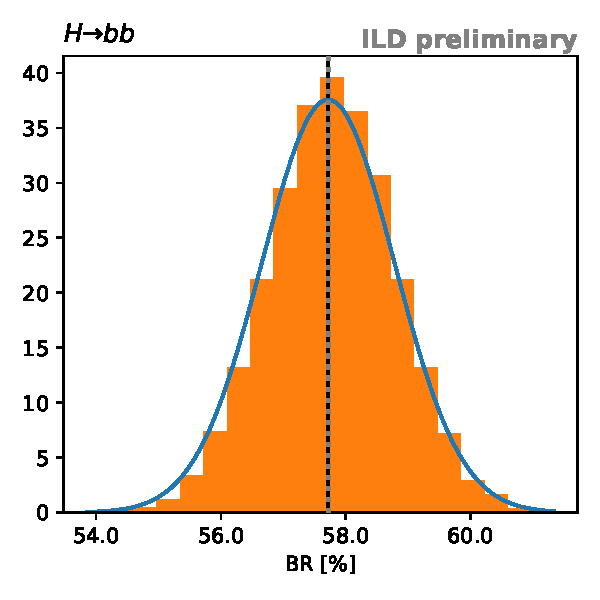
\includegraphics[height=0.7\textheight, keepaspectratio]
        {toys_default_bb}
    \end{column}
    \begin{column}{0.5\textwidth}
    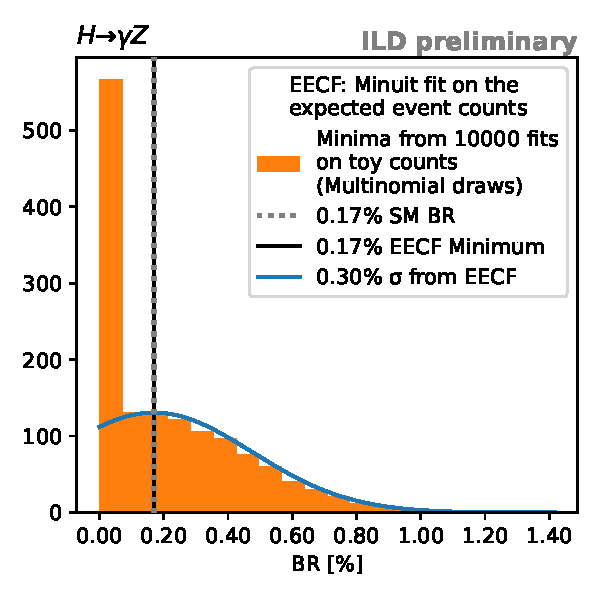
\includegraphics[height=0.7\textheight, keepaspectratio]
        {toys_default_az}
    \end{column}
    \end{columns}
    % \textit{\footnotesize
    %   For this slide only, we used $\texttt{MC1} = \texttt{MC2}$.
    %   $\texttt{MC1} \neq \texttt{MC2}$ shown in
    %   \emph{\ref{backup_bias_mc_limited} (backup).
    % }
    \end{frame}

    \begin{frame}{Fit in a non-SM scenario}
    \begin{columns}[b, onlytextwidth]
    \begin{column}{0.6\textwidth}
        \begin{tikzpicture}[remember picture,overlay]
            \node[anchor=west,inner sep=0pt] at ($(current page.west) + (0.15, 0)$) {
                \only<1>{
                    \begin{tabular}{rl}
                    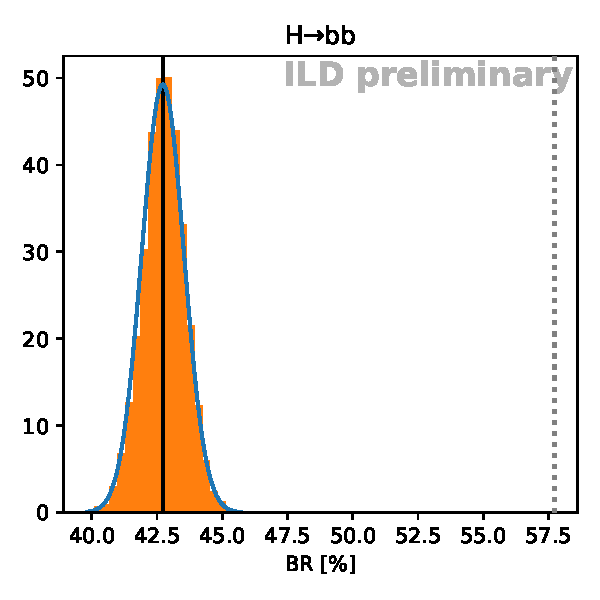
\includegraphics[width=0.45\textwidth]
                        {changed_toy_H_bb} &
                    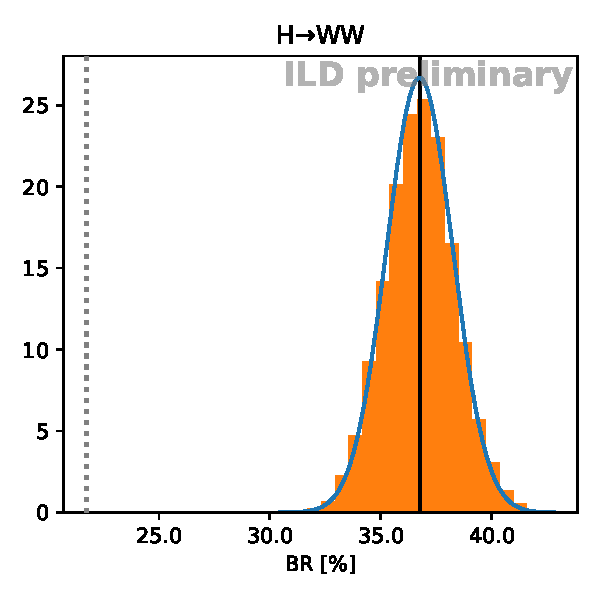
\includegraphics[width=0.45\textwidth]
                        {changed_toy_H_WW}
                    \end{tabular}
                }};
            \node[anchor=west,inner sep=0pt] at ($(current page.west) + (0.5, 0)$) {
                \only<2>{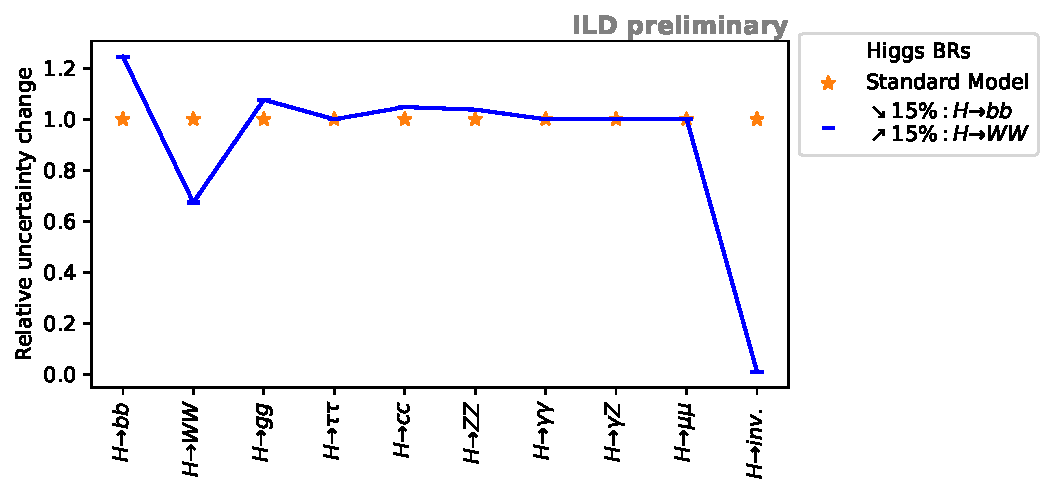
\includegraphics[width=\textwidth, keepaspectratio]
                {comparison_br_scenarios_1}}};
            \node[anchor=west,inner sep=0pt] at ($(current page.west) + (0.5, 0)$) {
                \only<3>{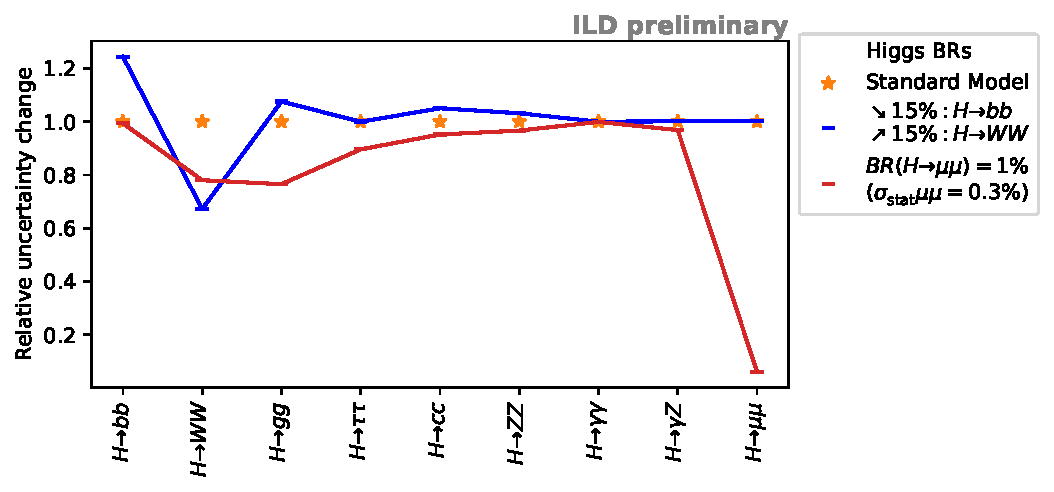
\includegraphics[width=\textwidth, keepaspectratio]
                {comparison_br_scenarios_2}}};
    \end{tikzpicture}
        Assume $57.7\% \to 42.7\%$ $BR(H\to b\bar{b})$, \\
        \hspace{4em}$21.8\% \to 36.8\%$ $BR(H\to W^+W^-)$.
    \end{column}
    \begin{column}{0.38\textwidth}
    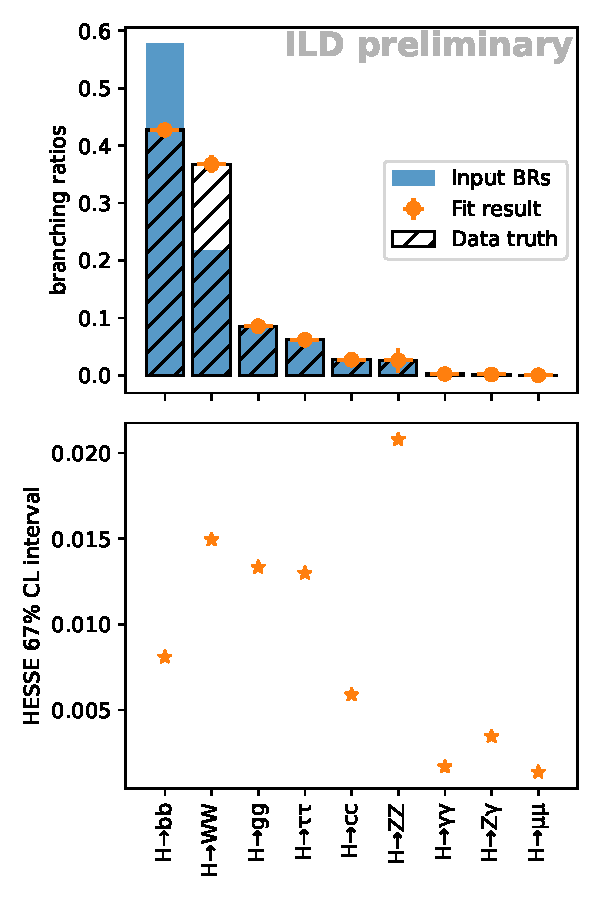
\includegraphics[height=0.85\textheight, keepaspectratio]
        {changed_br_estimates}
    \end{column}
    \end{columns}
    \end{frame}

    \begin{frame}{Dependency on polarization and background level}
    \begin{columns}[c, onlytextwidth]
    \begin{column}{0.5\textwidth}
    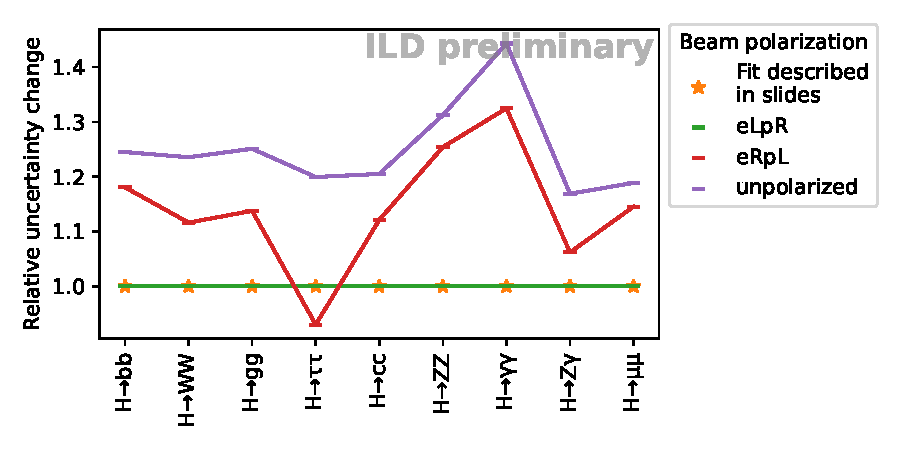
\includegraphics[width=\textwidth, keepaspectratio]
        {comparison_polarizations}
    \end{column}
    \begin{column}{0.5\textwidth}
        \only<1>{\put(0,0){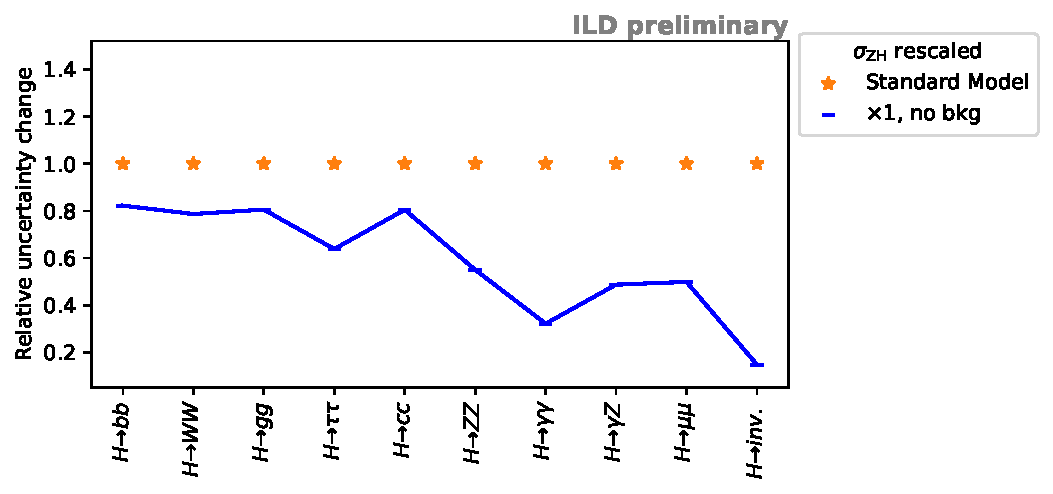
\includegraphics[width=\textwidth, keepaspectratio]{comparison_signal_scaler_partial}}}
        \only<2>{\put(0,0){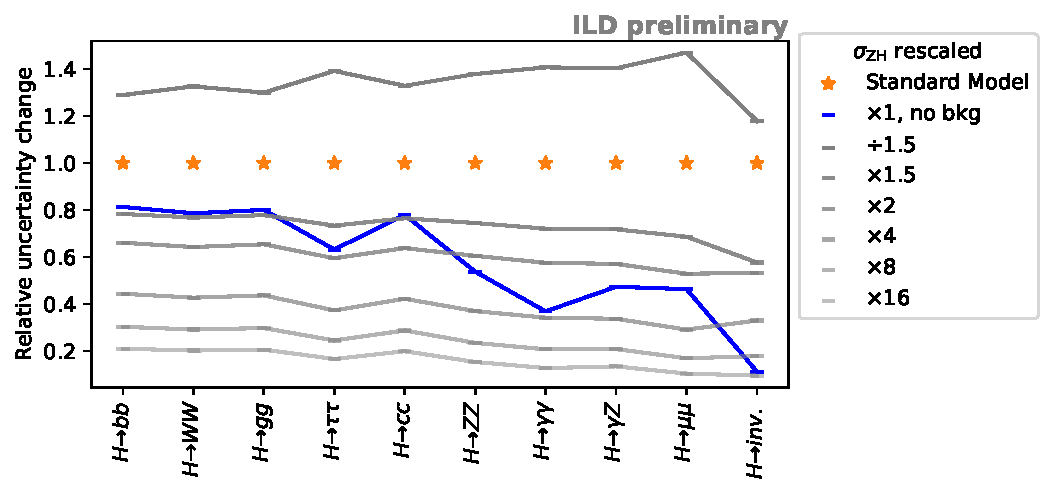
\includegraphics[width=\textwidth, keepaspectratio]{comparison_signal_scaler}}}
    \end{column}
    \end{columns}
    \end{frame}

\xsection{myblue}{Conclusion}
    \begin{frame}{Conclusions}
    \begin{columns}[c, onlytextwidth]
    \begin{column}{0.53\textwidth}
    \begin{itemize}
        \item[$-$] More work needed:
            \begin{itemize}
                \item[-] Better categories.
                \item[-] Exotic Higgs decays.
                % \item[-] Additional signal channels
                %     with decay-\-dependent selection efficiency \\
                %     (e.g. $ZH\to \nu \bar{\nu}H$).
            \end{itemize}
        \item[$+$] Extraction of major branching ratios\\
                from single analysis.
            \begin{itemize}
                \item[$\rightarrow$] Correlation matrix.
            \end{itemize}
        \item[$+$] Independent of $\sigma_{ZH}$ and $\sigma_{\tn{VV-fusion}}$.
        \item[$+$] Can automatically adapt to BR scenarios
            drastically different from SM.
        %v\item[$+$] Uncertainties look promising.
            % See {\color{llblue}\ref{comparison_with_global}} in backup.
    \end{itemize}
    \end{column}
    \begin{column}{0.02\textwidth}
    \end{column}
    \begin{column}{0.45\textwidth}
    \begin{table}
        \caption{Results of a fit on the
            expected event counts. In percent. ILD preliminary.}
        %\resizebox{\textwidth}{!}{
            \InputBiasTable{bias_table_default.tex}
    %}
    \end{table}
    \end{column}
    \end{columns}
    \end{frame}


\newcounter{finalframe}\setcounter{finalframe}{\value{framenumber}}
\xsection{myblue}{Back-up}[pr_ilc_cavity_resized]
    \begin{frame}{Expected counts per (category, BR) pair}
    \begin{columns}[c, onlytextwidth]
    \begin{column}{0.5\textwidth}
        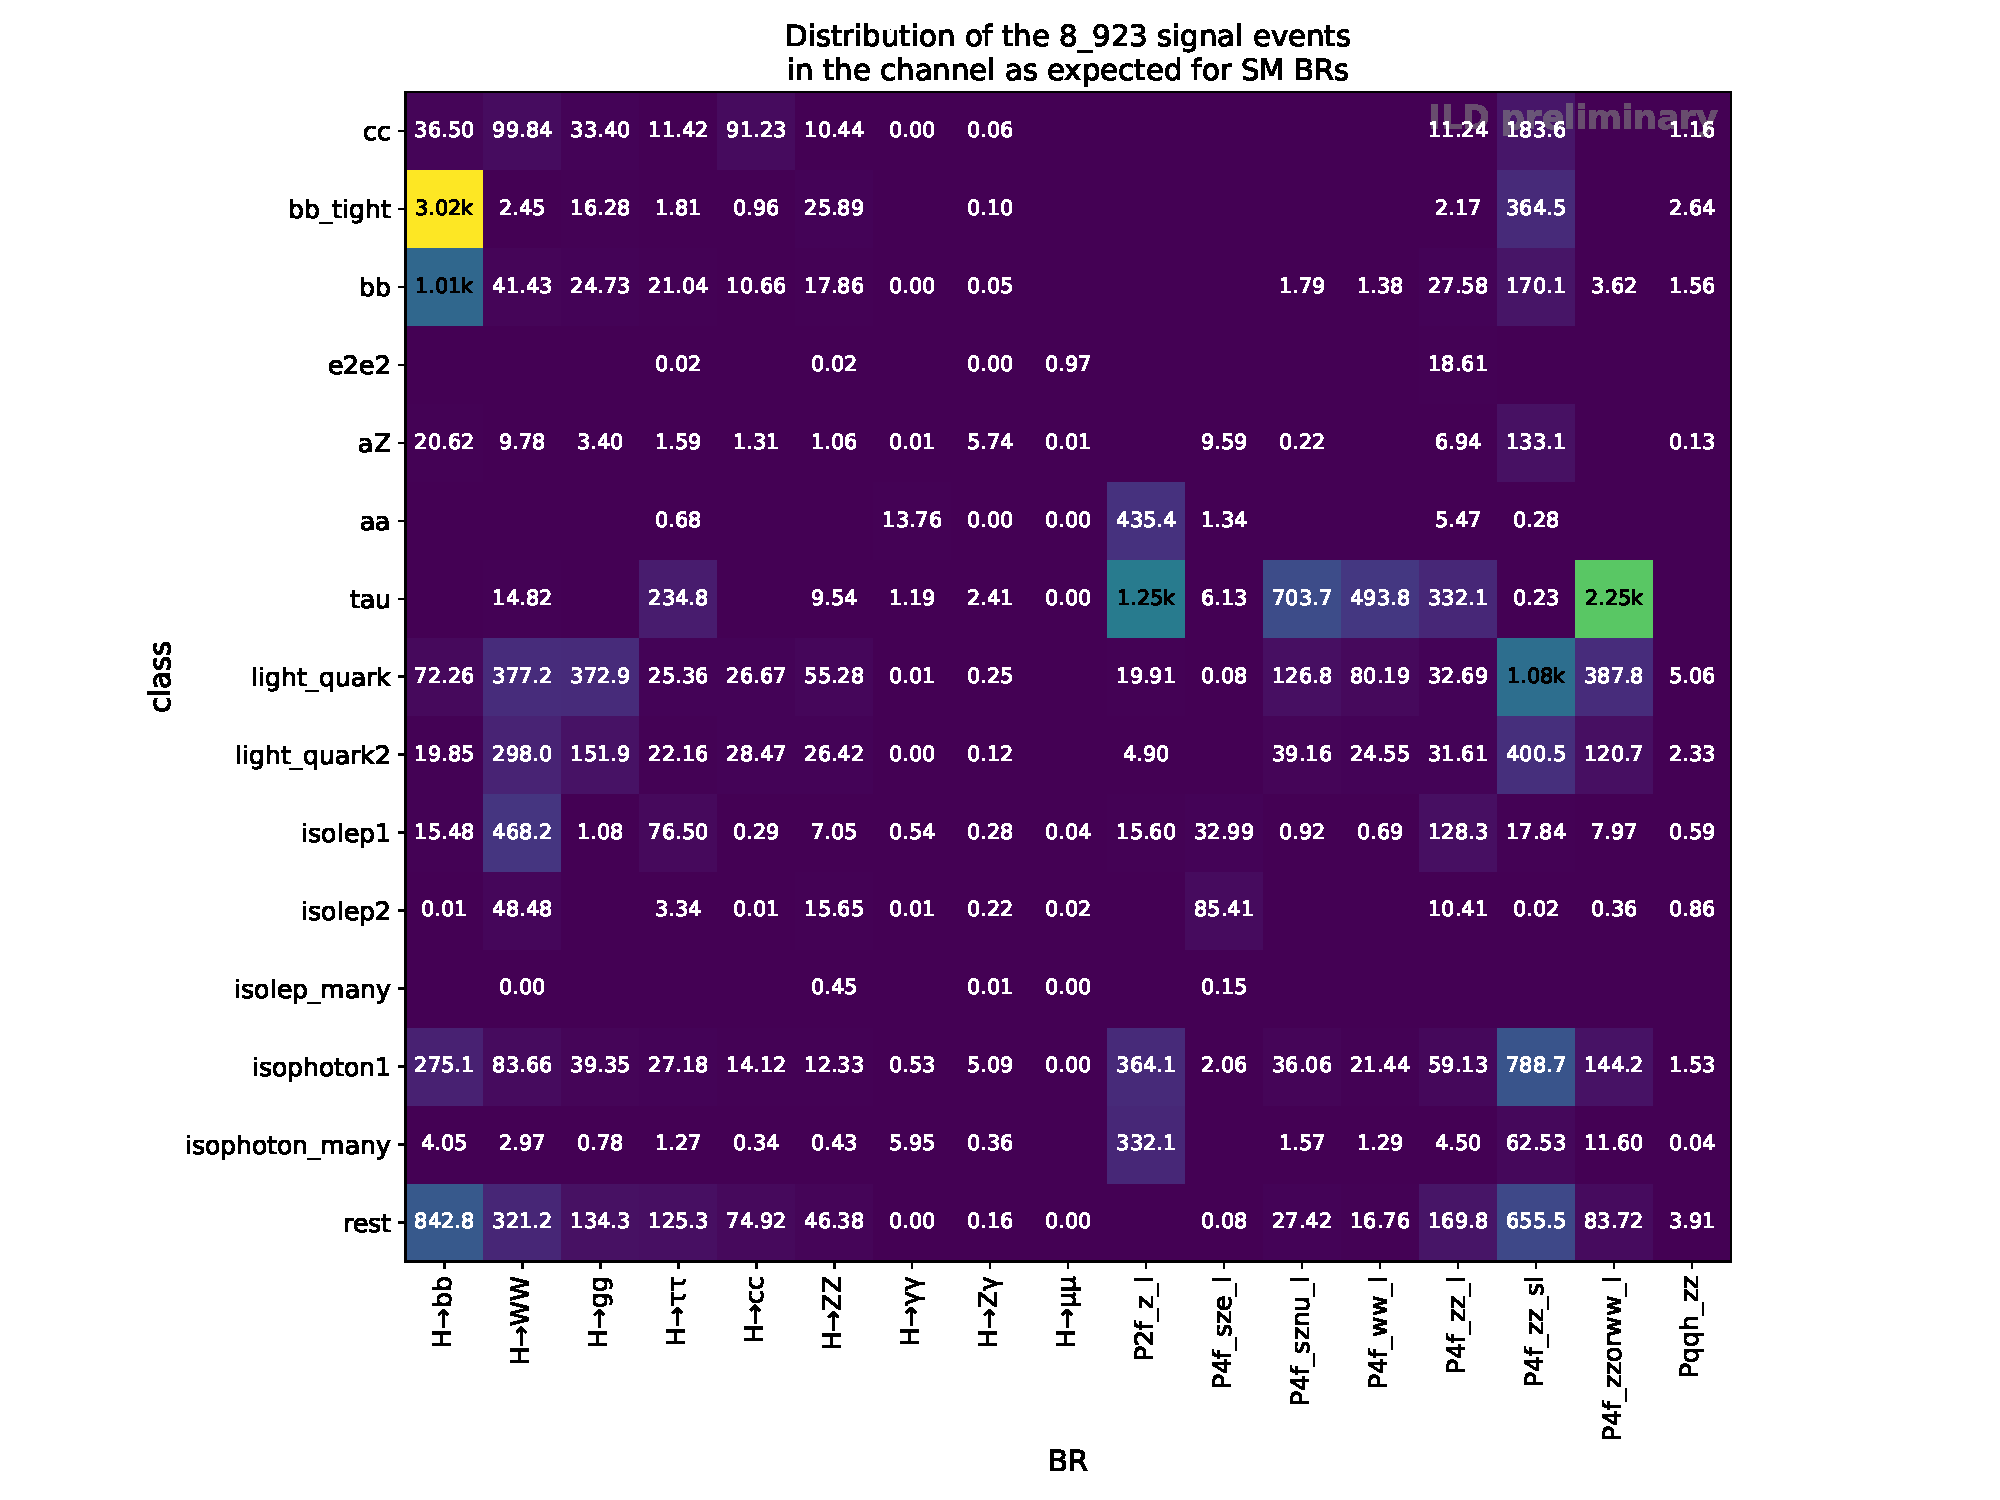
\includegraphics[height=0.9\textheight, width=0.95\textwidth, keepaspectratio]
        {expected_counts_matrix_bkg_e2e2}
    \end{column}
    \begin{column}{0.5\textwidth}
        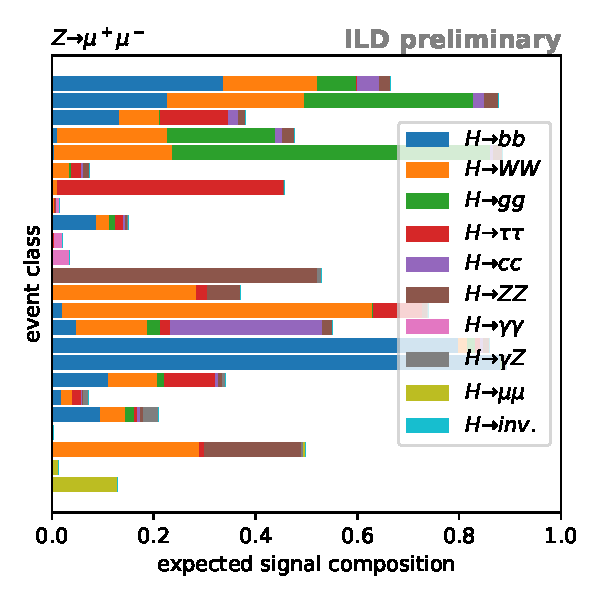
\includegraphics[height=0.9\textheight, width=0.95\textwidth, keepaspectratio]
        {intro_signal_composition_per_category_w_bkg}
    \end{column}
    \end{columns}
    \end{frame}

    \begin{frame}{BR correlations with the current categories}
    \label{correlations}
    Higher correlations motivate improvements in the category definition.
    Needed to include the results in a global fit.
    Also needed for the last BR:
    \begin{columns}[c, onlytextwidth]
        \begin{column}{0.4\textwidth}
        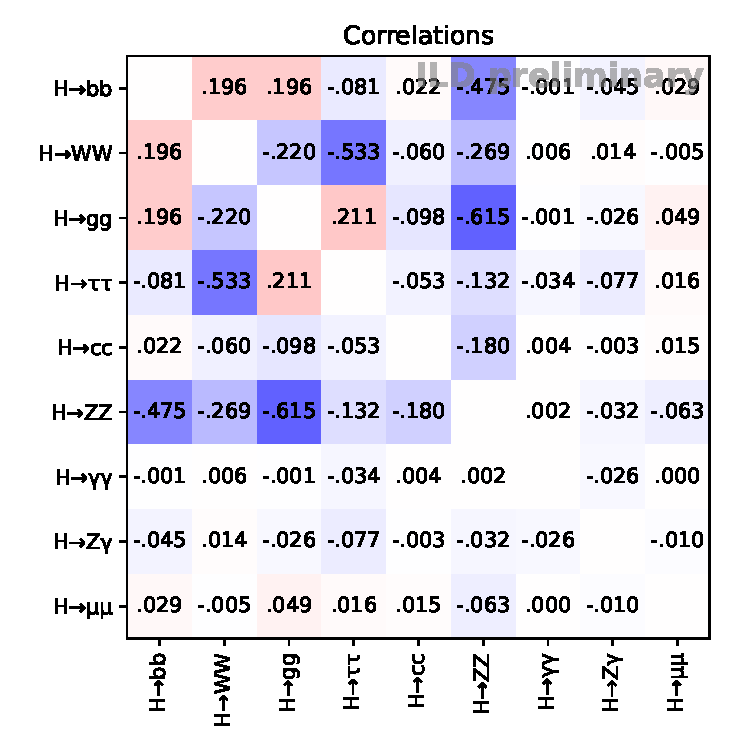
\includegraphics[height=0.7\textheight, width=\textwidth, keepaspectratio]
            {correlations}
        \end{column}
        \begin{column}{0.6\textwidth}
        {\footnotesize\begin{align*}
        B_{ZZ^*} = 1 - \sum_{\scriptscriptstyle i \neq ZZ^*} B_i
        \Rightarrow \sigma^2_{ZZ^*} =
        \sum_{\scriptscriptstyle i \neq ZZ^*}
        \sum_{\scriptscriptstyle j \neq ZZ^*}
        \rho_{ij} \sigma_i \sigma_j
        \end{align*}}
        \vspace{-0.75\baselineskip}
        \begin{center}
        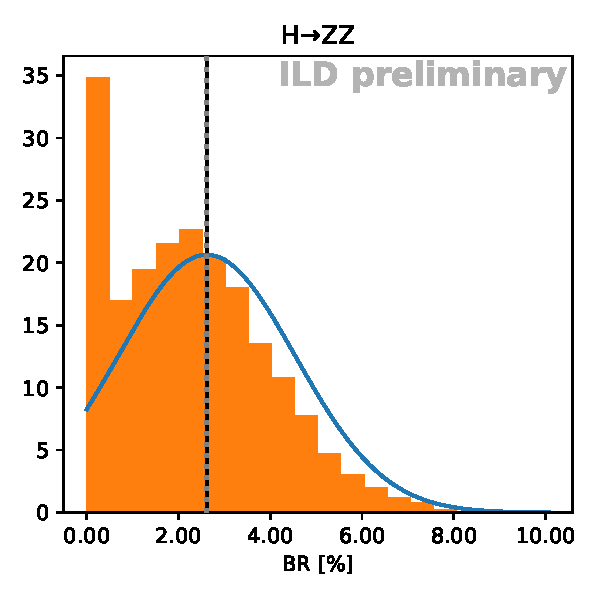
\includegraphics[height=0.6\textheight]
            {toy_H_ZZ}
        \end{center}
        \end{column}
    \end{columns}
    \end{frame}

    \begin{frame}{Comparison with global coupling fits}
    \label{comparison_with_global}
    \begin{columns}[c, onlytextwidth]
    \begin{column}{0.55\textwidth}
    \vspace{-0.2\baselineskip}
    \begin{itemize}
        \item {[1], [2]} use existing analyses and combine them
            to extract a combined sensitivity for the Higgs boson couplings.
        \item {[1]} scaled to the H-20 ILC250 scenario.
        \item \textit{This fit} is our approach.
        \begin{itemize}
            \item A single analysis
                  directly fitting the branching ratios to data.
            % \item Expressed as couplings for comparison.
            \item So far only $Z \to e^+ e^-$, $Z \to \mu^+ \mu^-$.
            \item Only statistical uncertainty.
        \end{itemize}
    \end{itemize}
    \end{column}
    \begin{column}{0.45\textwidth}
        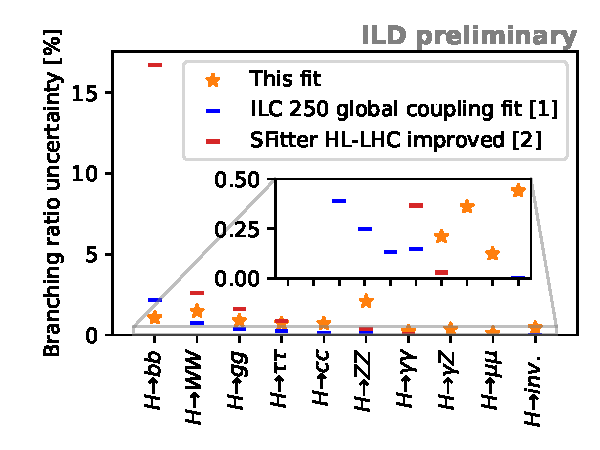
\includegraphics[width=\textwidth, keepaspectratio]
            {comparison_with_others}
    \end{column}
    \end{columns}
    \vspace{0.2\baselineskip}
    {\small
    [1] J.~Tian, K.~Fujii~\href{https://www.sciencedirect.com/science/article/pii/S2405601415006161}
        {\color{llblue} \textit{Measurement of Higgs boson couplings at the International Linear Collider}}.
    [2] SFitter~\href{https://inspirehep.net/literature/1209590}
        {\color{llblue} \textit{Measuring Higgs Couplings at a Linear Collider}}.
    }
    \end{frame}

    \begin{frame}%[shrink]
    \frametitle{Higgsstrahlung}
    \begin{columns}[c,onlytextwidth]
    \begin{column}{0.40\textwidth}
    \resizebox{\textwidth}{!}{\FeynmanHiggsstrahlung}
    \end{column}
    \begin{column}{0.60\textwidth}
    % Like locally setting the font size from 11 to 10.
    \setbeamertemplate{itemize/enumerate body begin}{\footnotesize}
    \setbeamertemplate{itemize/enumerate subbody begin}{\footnotesize}
    \vspace{-1\baselineskip} % Still in font size 10, it is one line too long.
    \begin{itemize}
        \item \textcolor{xemphcolor}{
            $Z \rightarrow \mu^+ \mu^-, Z \rightarrow e^+ e^-$}:

            Golden channels due to recoil mass method,
            $M_{\tn{recoil}}^2 = s + M_Z^2 - 2\sqrt{s} \cdot E_Z$.
        \item \textcolor{xemphcolor}{
            $Z \rightarrow \tau^+ \tau^-$}:

            Event tagging on the $\tau$ is complicated.
            \begin{itemize}
                \item Large $\tau$ decay opening angle (low $E_\tau$).
                \item Divers environment from the Higgs decay.
            \end{itemize}
        \item \textcolor{xemphcolor}{
            $Z \rightarrow \nu\bar{\nu}$}:
            \begin{itemize}
                \item[--] Significant WW-fusion contribution in $\nu\bar{\nu}H$.
                \item[--] Cannot tag event on $\nu$.
                \item[+]  Only Higgs boson (and beam overlay) in event.
                \item[+]  $6\times$ higher cross section.
            \end{itemize}

        \item \textcolor{xemphcolor}{
            $Z \rightarrow q \bar{q}$}:
            \begin{itemize}
                \item[+]  Hightest cross section.
                \item[--] Hard to identify the traces from the Z decay
                    without making assumptions on the Higgs decay.
            \end{itemize}
    \end{itemize}
    \end{column}
    \end{columns}
    \end{frame}

    \begin{frame}
    \frametitle{Example events}
    After removing the primary Z boson,
    the \textit{signal} events per channel are interchangeable.
    \centering
    \begin{tabular}{cc}
        \begin{tikzpicture}
          \node (img1) {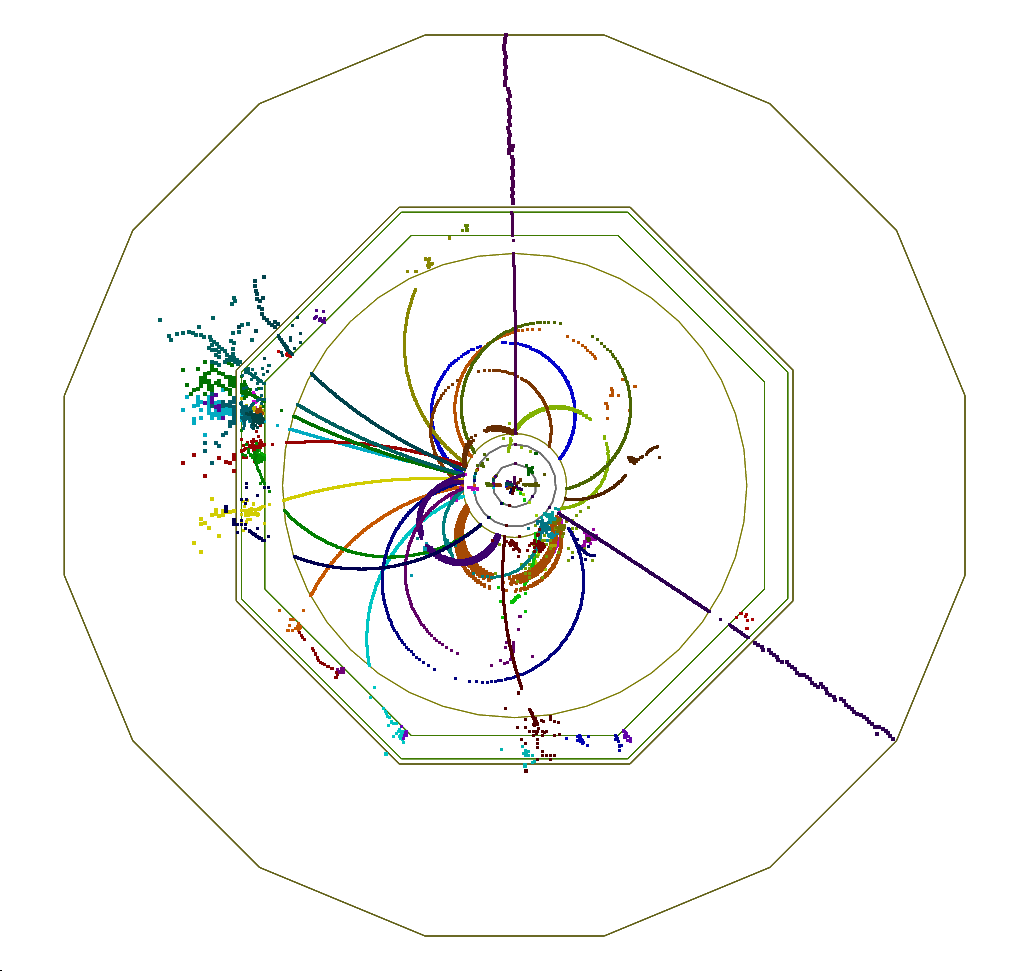
\includegraphics[height=0.65\textheight]{pr_frontview-70}};
          \node (img2) at (img1) {\only<2->{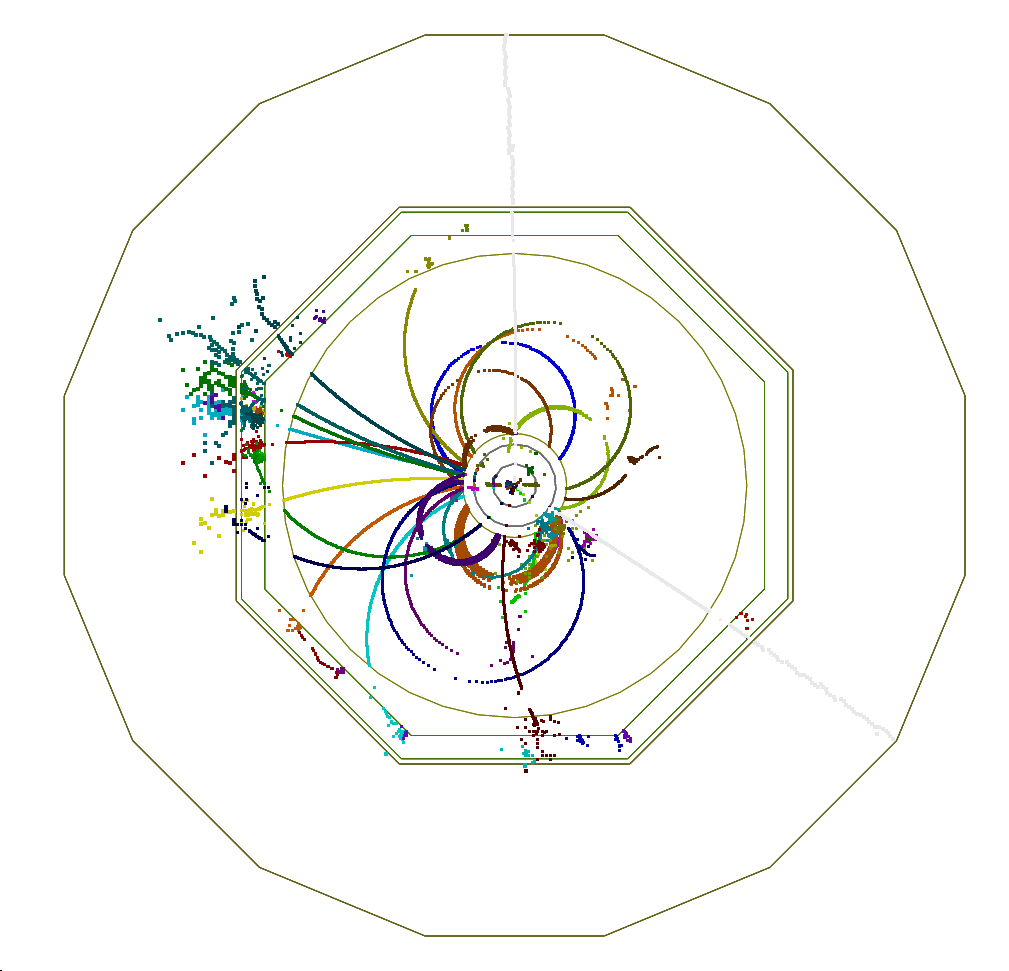
\includegraphics[height=0.65\textheight]{pr_frontview-70_noMu}}};
        \end{tikzpicture} &

        \begin{tikzpicture}
          \node (img1) {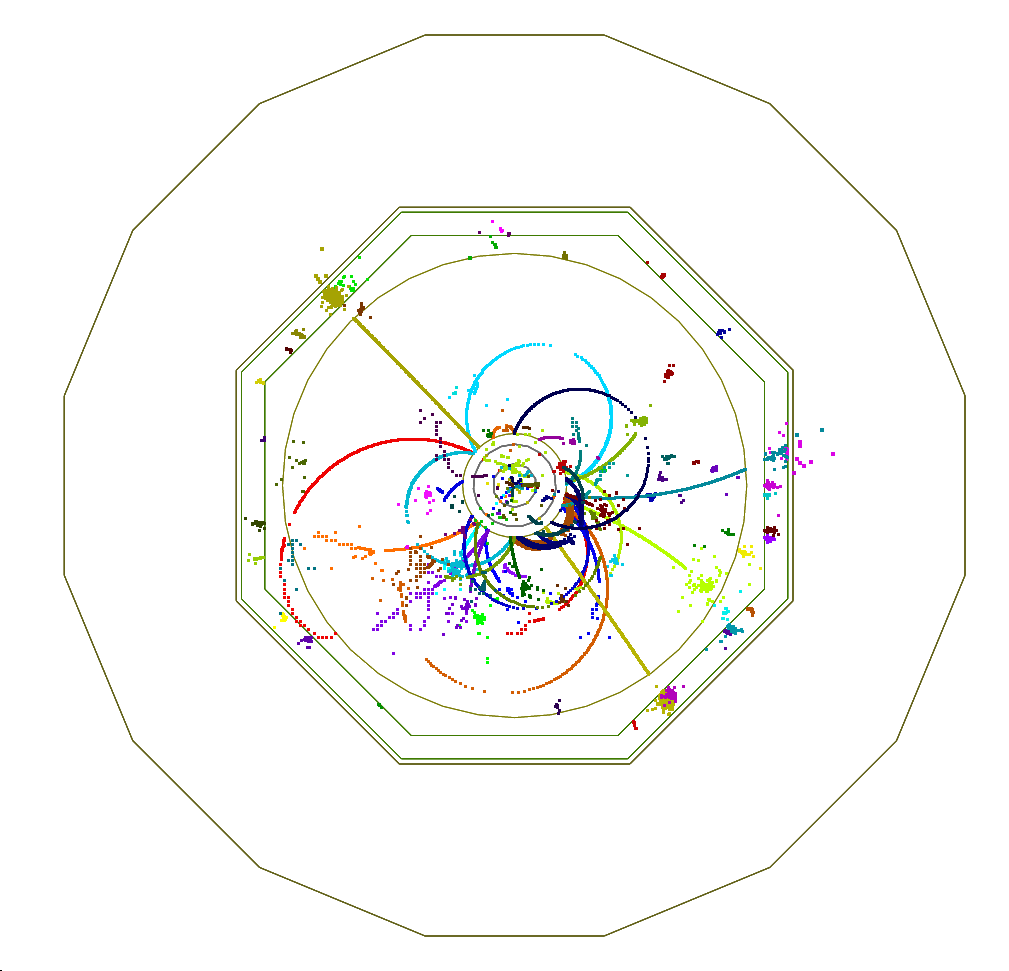
\includegraphics[height=0.65\textheight]{pr_frontview-91}};
          \node (img2) at (img1) {\only<3->{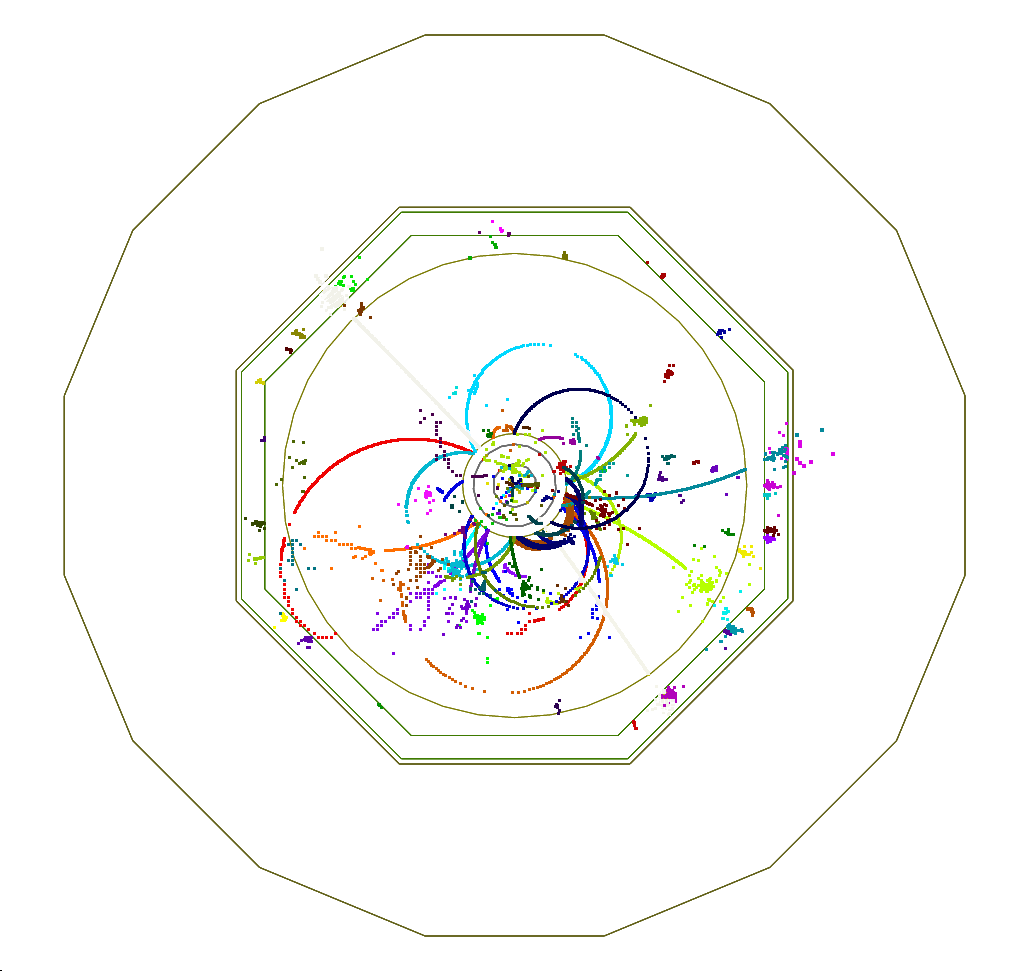
\includegraphics[height=0.65\textheight]{pr_frontview-91_noEl}}};
          \node (img2) at (img1) {\only<4->{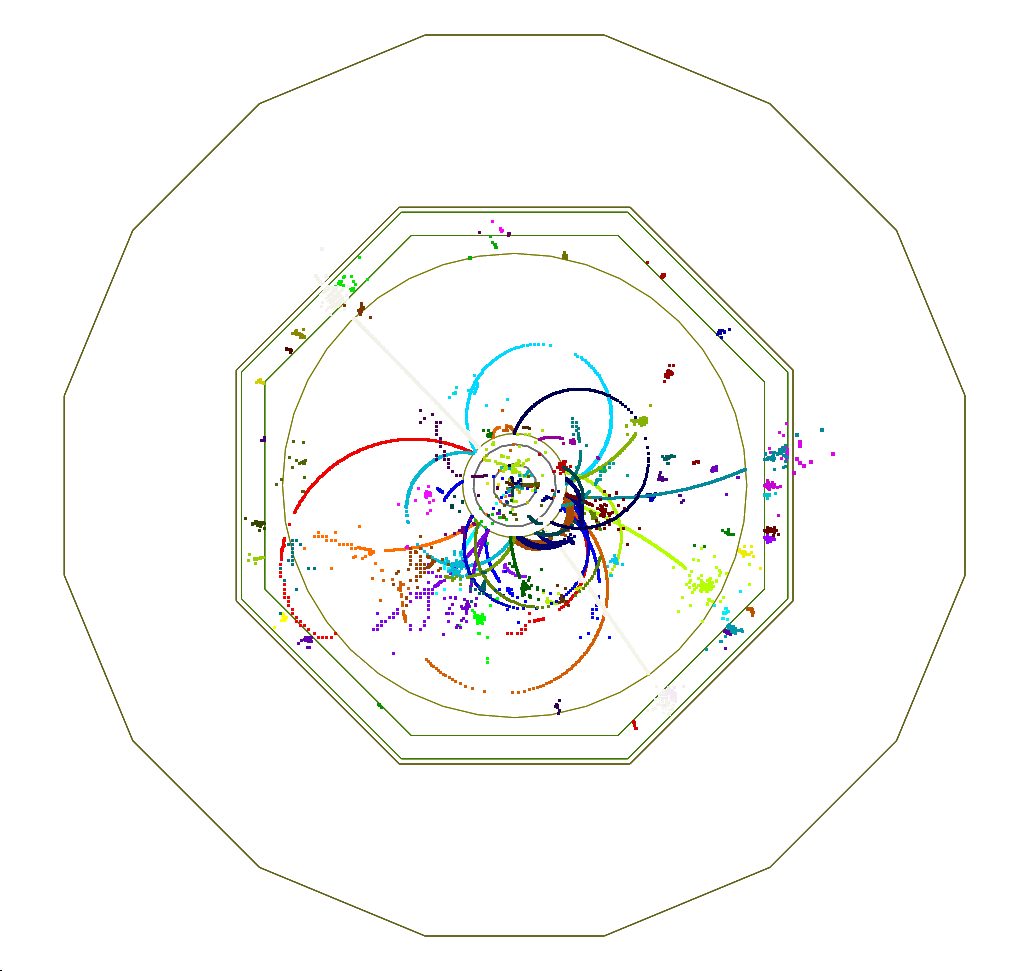
\includegraphics[height=0.65\textheight]{pr_frontview-91_noElGamma}}};
        \end{tikzpicture} \\
        \footnotesize{$e^+e^- \rightarrow H$
            \onslide<1>{$Z, \ Z \rightarrow \mu^+ \mu^-$}
        } &
        \footnotesize{$e^+e^- \rightarrow H$
            \onslide<-2>{$Z, \ Z \rightarrow e^+ e^-$}
        } \\
    \end{tabular}
    \end{frame}

\setcounter{framenumber}{\value{finalframe}}
\end{document}
